\chapter{AVALIAÇÃO E RESULTADOS}
\label{chap:avaliacao}

Este capítulo apresenta a avaliação experimental e a análise dos resultados obtidos nos três protótipos desenvolvidos para validar a arquitetura \nome\ e compará-la ao protocolo \polka\ original. Seguindo a estratégia incremental detalhada no Capítulo~\ref{chap:prototipos}, os ensaios exploram desde a seleção explícita de caminhos em hardware programável de alta capacidade até o fatiamento conjunto de rotas e políticas de enfileiramento em planos de dados emulados em P4 e acelerados via eBPF/XDP no \textit{kernel} Linux.

% ==============================================================================
\section{Metodologia Experimental e Métricas Avaliadas}
\label{sec:metodologia_avaliacao}

Para avaliar de forma abrangente a eficácia do isolamento de recursos, a previsibilidade de atraso e a agilidade na reconfiguração dinâmica das fatias de rede sem manutenção de estados no núcleo, os experimentos foram organizados em três frentes complementares:

\begin{itemize}
    \item \textbf{Protótipo 1 (\textit{Testbed} PORVIR -- Hardware Intel Tofino/freeRtr):} avalia o fatiamento baseado exclusivamente na seleção explícita de caminhos fim a fim no \polka\ original sobre enlaces físicos interestaduais de 10~Gbit/s;
    \item \textbf{Protótipo 2 (Emulação P4/BMv2 com \textit{Traffic Manager} WDRR):} valida o encapsulamento unificado de rota e fila (\routeID) do \nome\ em enlaces de 10~Mbit/s, verificando o isolamento ponderado de banda e a migração dinâmica de políticas em duas rodadas experimentais;
    \item \textbf{Protótipo 3 (Virtualização Containerlab com eBPF/XDP e Linux \texttt{tc}):} investiga o comportamento do \nome\ em enlaces de 1~Gbit/s sob cargas heterogêneas multiserviço (fluxos UDP sensíveis a atraso e fluxos TCP elásticos), comparando progressivamente os escalonadores FIFO, WDRR e SP-WDRR, bem como os algoritmos de controle de congestionamento CUBIC e BBR.
\end{itemize}

Na geração de cargas de trabalho e instrumentação das medições, empregou-se a ferramenta \texttt{iperf3} para injeção de fluxos TCP e UDP e aferição de vazão efetiva, \textit{jitter} (conforme RFC~3550), taxa de perda e volume de retransmissões TCP, além de sondas ICMP (\texttt{ping}) para monitoramento contínuo do tempo de ida e volta (RTT) médio, máximo e de cauda (95º percentil). Nos ensaios do Protótipo~3, também foram coletadas estatísticas internas diretamente das disciplinas de enfileiramento do subsistema \texttt{tc} do \textit{kernel} Linux (ocupação de \textit{buffer}/\textit{backlog} e contagem de pacotes por fila salto a salto).

% ==============================================================================
\section{Protótipo 1 -- PolKA Original em Hardware Programável}
\label{sec:res_prototipo1}

O primeiro protótipo foi avaliado no \textit{testbed} nacional PORVIR~\cite{Nogueira2025}, composto por quatro nós implementados em comutadores programáveis Intel Tofino\textregistered\ gerenciados pelo plano de controle \texttt{freeRtr}\footnote{\url{http://www.freertr.org/}} (topologia ilustrada na Figura~\ref{fig:porvir_topo}). Para avaliar individualmente o desempenho das rotas disponíveis entre Vitória e São Paulo, foram provisionados três túneis \polka\ distintos: \texttt{VIX--RJ--SP}, \texttt{VIX--MG--SP} e \texttt{VIX--RJ--MG--SP}.

\subsection{Caracterização de Desempenho dos Caminhos}
\label{subsec:porvir_caracterizacao}

Inicialmente, caracterizou-se o desempenho basal de cada rota em termos de latência média, vazão média e volume de retransmissões, conforme sintetizado na Tabela~\ref{tab:metricas_porvir}. As medições de tráfego TCP foram conduzidas via \texttt{iperf3} durante 60 minutos para cada caminho, com amostragens coletadas a cada 30 segundos, enquanto o RTT médio foi aferido por meio de sondas ICMP (\texttt{ping}) em intervalos de 1 segundo ao longo do mesmo período.

\begin{table}[htbp]
\centering
\caption{Métricas de desempenho por caminho no \textit{testbed} PORVIR (Protótipo 1).}
\label{tab:metricas_porvir}
\begin{tabularx}{\textwidth}{Xccc}
\toprule
\textbf{Caminho} & \textbf{Latência média} & \textbf{Vazão média} & \textbf{Retransmissões (pacotes)} \\
\midrule
\texttt{VIX--RJ--SP}     & 13~ms & 38,610~Gbit/s & 998 \\
\texttt{VIX--MG--SP}     & 17~ms & 0,829~Gbit/s  & 186.327 \\
\texttt{VIX--RJ--MG--SP} & 26~ms & 0,787~Gbit/s  & 244.680 \\
\bottomrule
\end{tabularx}
\fonte{Elaborado pelo autor (2026).}
\end{table}

Os resultados evidenciam que o caminho principal \texttt{VIX--RJ--SP} apresenta desempenho substancialmente superior aos demais, registrando vazão média aproximadamente 46 vezes maior (38,610~Gbit/s), menor atraso médio (13~ms) e número reduzido de retransmissões (998 pacotes), ao passo que \texttt{VIX--MG--SP} e \texttt{VIX--RJ--MG--SP} atuam como rotas alternativas de menor capacidade.

\subsection{Isolamento e Migração Dinâmica de Fatias}
\label{subsec:porvir_migracao}

Após a etapa de caracterização, executou-se um experimento com três fluxos TCP concorrentes gerados via \texttt{iperf3} sobre o enlace de alta capacidade (\texttt{VIX--RJ--SP}), representando a coexistência entre uma fatia de rede prioritária (Fluxo~1) e duas fatias de menor prioridade (Fluxos~2 e~3). Nesse cenário, cada fluxo opera como uma fatia independente, recebendo recursos isolados e sendo reconfigurado dinamicamente na borda conforme seus requisitos de QoS.

\begin{figure}[htbp]
    \centering
    \captionsetup{justification=centering}
    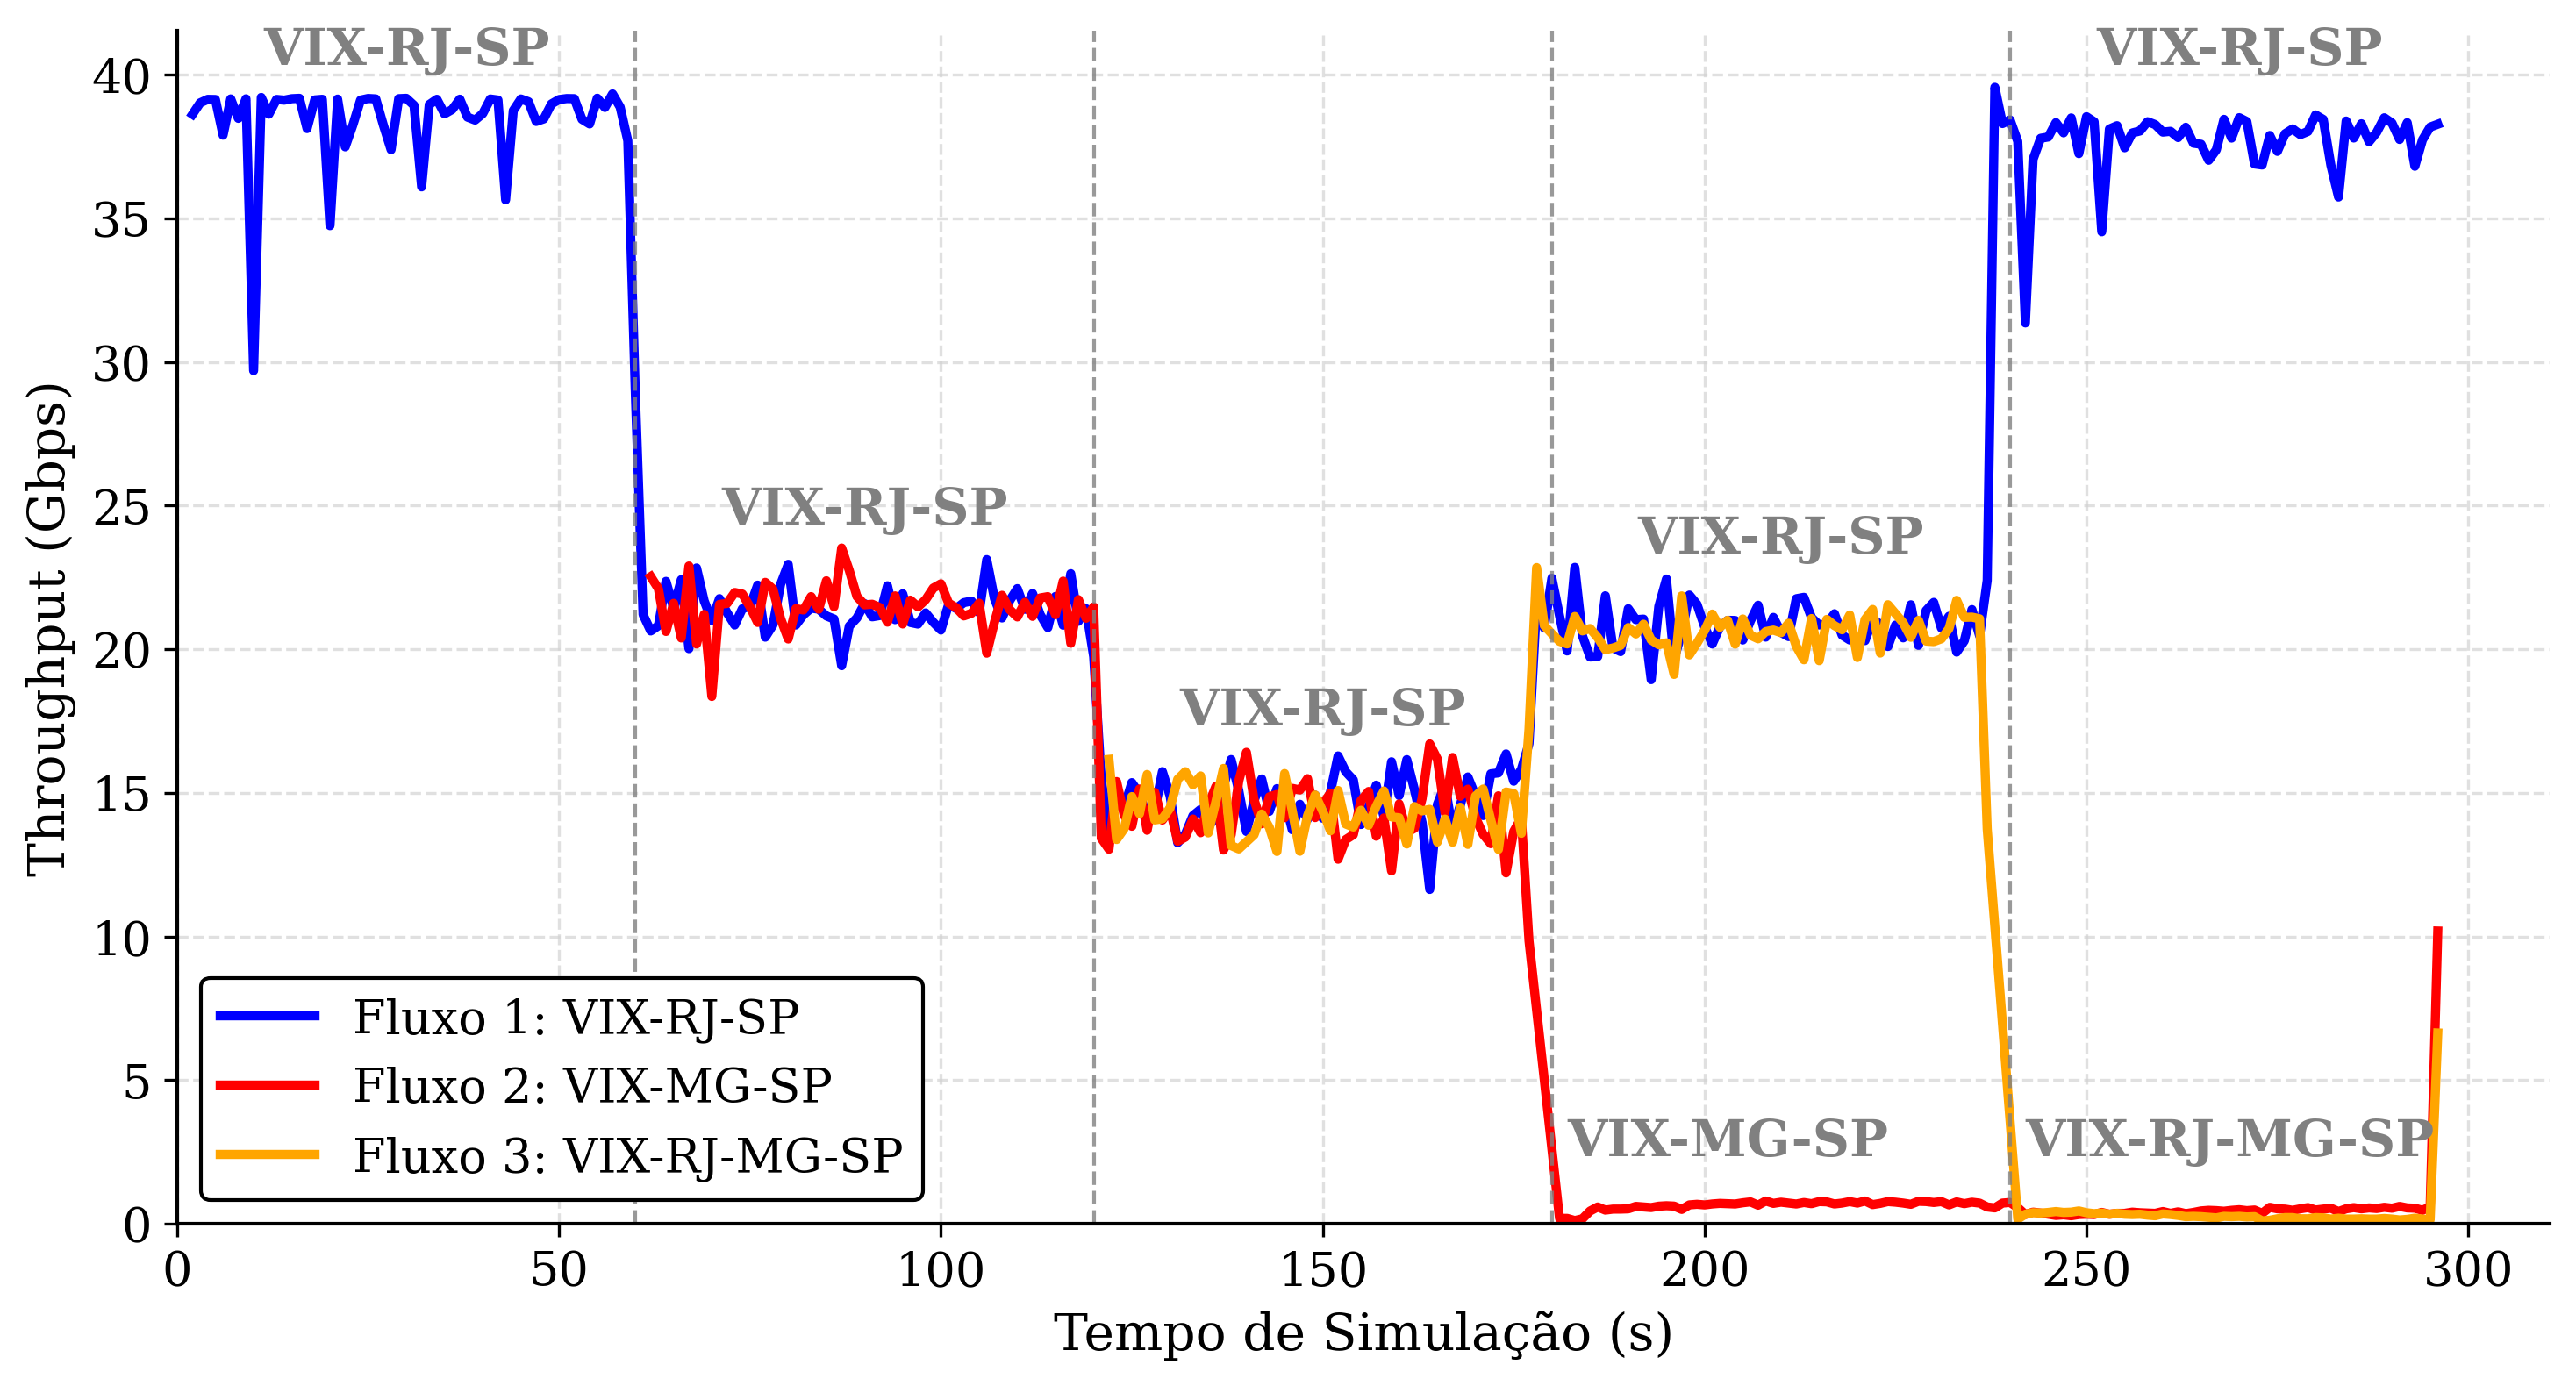
\includegraphics[width=0.85\linewidth]{figuras/grafico_mudanca_caminho_porvir.png}
    \caption{Evolução temporal da vazão e migração dinâmica de caminhos no \textit{testbed} PORVIR (Protótipo 1).}
    \label{fig:porvir_vazao}
\end{figure}

A Figura~\ref{fig:porvir_vazao} apresenta a evolução temporal da vazão coletada ao longo dos eventos, espaçados em intervalos de 60 segundos e divididos em duas fases principais:

\begin{itemize}
    \item \textbf{Fase de competição ($0 \le t < 180\text{~s}$):} a fatia correspondente ao Fluxo~1 inicia operando isoladamente no caminho principal (\texttt{VIX--RJ--SP}), alcançando cerca de 38,6~Gbit/s. Nos instantes $t = 60\text{~s}$ e $t = 120\text{~s}$, as fatias concorrentes dos Fluxos~2 e~3 são ativadas sobre a mesma rota, passando a disputar a largura de banda do enlace e reduzindo a taxa efetiva de cada fluxo para aproximadamente 21~Gbit/s (com dois fluxos) e 14~Gbit/s (com três fluxos).
    \item \textbf{Fase de migração ($180 \le t \le 300\text{~s}$):} demonstrando o isolamento lógico e a adaptação dinâmica proporcionados pelo roteamento na origem, as fatias concorrentes são realocadas para rotas alternativas de menor capacidade sem necessidade de reconfiguração nos comutadores intermediários. O Fluxo~2 é migrado para o caminho \texttt{VIX--MG--SP} em $t = 180\text{~s}$, enquanto o Fluxo~3 é redirecionado para \texttt{VIX--RJ--MG--SP} em $t = 240\text{~s}$. Como resultado, a fatia prioritária do Fluxo~1 restabelece integralmente o uso da capacidade do enlace principal.
\end{itemize}

Apesar da eficácia demonstrada na seleção de rotas, o \polka\ original atua estritamente no nível de caminho, não oferecendo diferenciação por filas dentro de um mesmo enlace compartilhado --- limitação superada pela arquitetura \nome\ avaliada nos protótipos subsequentes.

% ==============================================================================
\section{Protótipo 2 -- SPolKA em Plano de Dados P4/BMv2}
\label{sec:res_prototipo2}

O segundo protótipo valida a arquitetura \nome\ em ambiente emulado (Mininet/BMv2) sobre a topologia da Figura~\ref{fig:topologia_polka}, na qual o identificador \routeID\ codifica simultaneamente a trajetória e a fila de escalonamento em cada salto. Conforme detalhado na Seção~\ref{sec:prototipo_bmv2}, cada interface de egresso dos roteadores de núcleo opera com enlaces de 10~Mbit/s e duas filas gerenciadas pelo \textit{Traffic Manager} customizado com algoritmo WDRR~\cite{Elbediwy2025}: a \textbf{Fila~1} (prioritária, com reserva de 70\% da banda) e a \textbf{Fila~2} (secundária, com reserva de 30\% da banda). Os fluxos de dados entre clientes ($H_i$) e servidores ($S_i$) foram gerados via \texttt{iperf3} utilizando o protocolo TCP em duas rodadas experimentais.

\subsection{Primeira Rodada -- Reconfiguração Dinâmica de Políticas de Filas}
\label{subsec:prot2_rodada1}

Na primeira rodada experimental, investigou-se exclusivamente o impacto da alteração dinâmica de filas sobre um mesmo caminho físico (\texttt{\{C1, C3, C5, C6\}}). Foram instanciadas três fatias de rede: uma fatia de alta prioridade, representada pelo fluxo $H_3 \rightarrow S_3$, e duas fatias de menor prioridade, representadas pelos fluxos $H_4 \rightarrow S_4$ e $H_5 \rightarrow S_5$, visando validar o isolamento de recursos em condições de saturação do enlace.

\begin{figure}[htbp]
    \centering
    \captionsetup{justification=centering}
    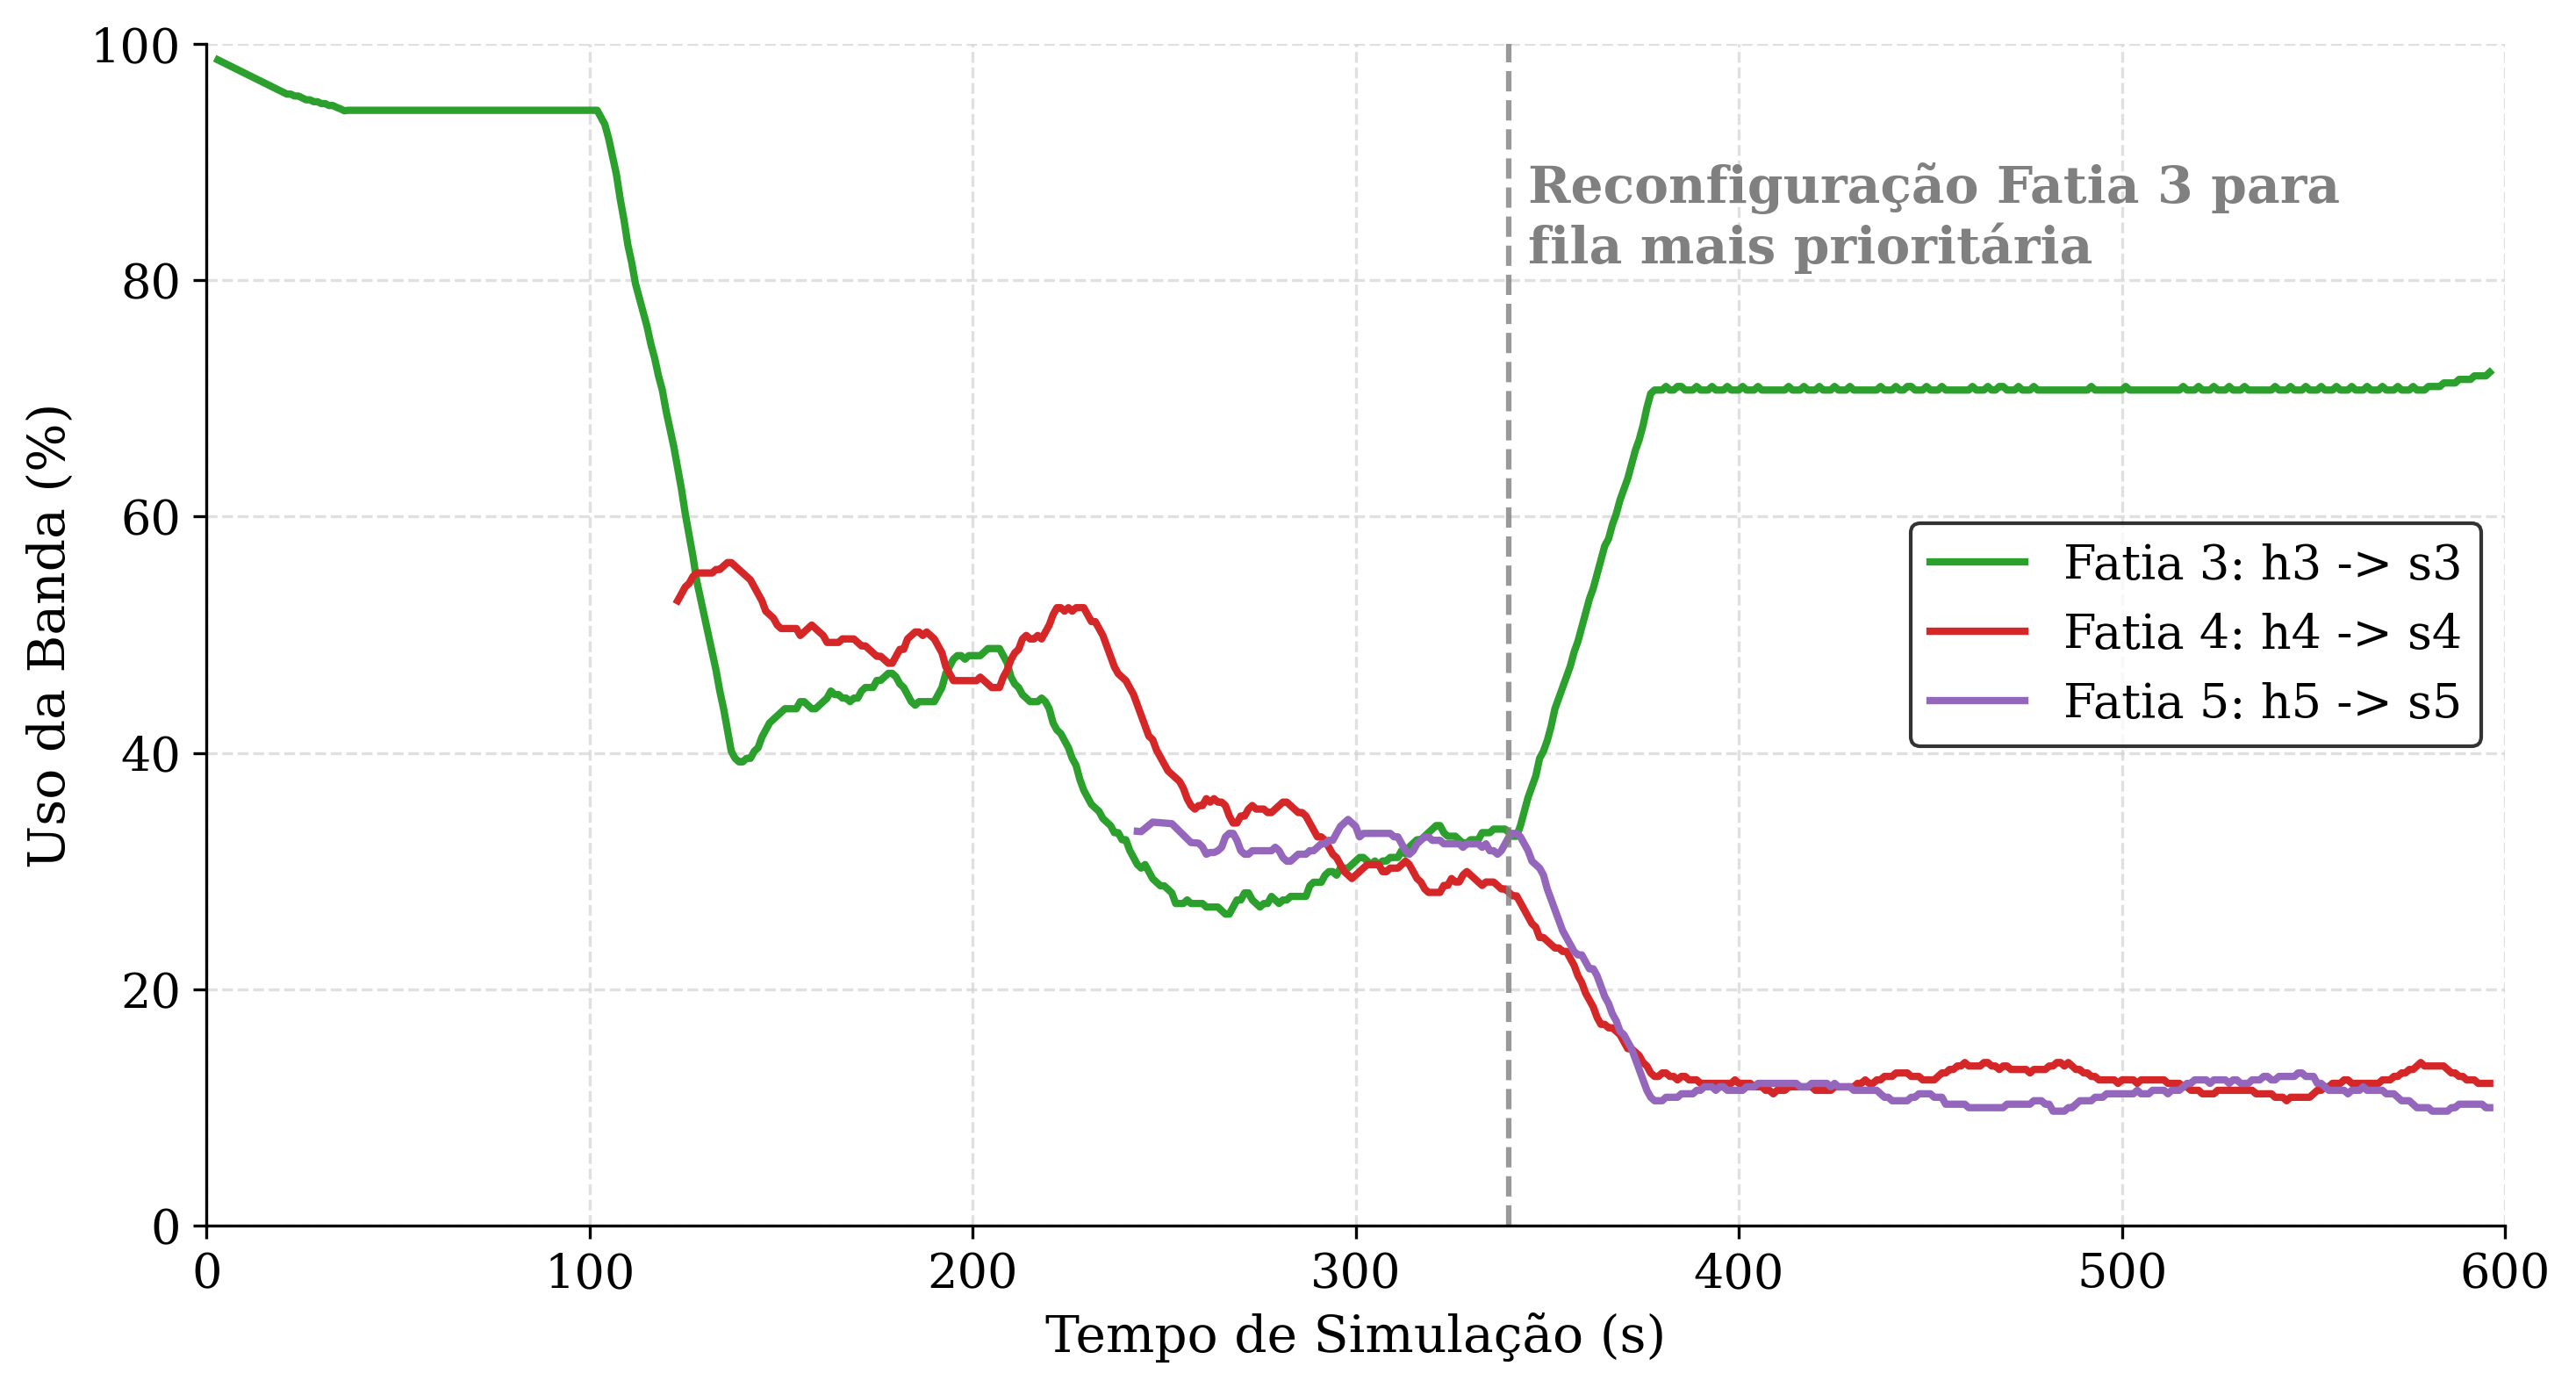
\includegraphics[width=0.85\linewidth]{figuras/grafico_mudanca_fila_polka.png}
    \caption{Ocupação de banda na primeira rodada do Protótipo 2: reconfiguração dinâmica da Fatia 3 para a fila prioritária.}
    \label{fig:mininet_mudanca_fila_polka}
\end{figure}

Conforme ilustrado na Figura~\ref{fig:mininet_mudanca_fila_polka}, o ensaio desenvolve-se em duas etapas principais:
\begin{itemize}
    \item \textbf{Compartilhamento inicial na fila secundária:} no início da execução, o fluxo $H_3 \rightarrow S_3$ (Fatia~3) é alocado na \textbf{Fila~2} em todos os saltos. Pela propriedade de conservação de trabalho (\textit{work-conserving}) do algoritmo WDRR, na ausência de tráfego na fila prioritária, a largura de banda total disponível no enlace é usufruída pela Fila~2. Com a entrada sequencial dos fluxos concorrentes $H_4 \rightarrow S_4$ (Fatia~4) e $H_5 \rightarrow S_5$ (Fatia~5) na mesma fila, a capacidade do enlace passa a ser dividida de forma equitativa entre as três fatias (cerca de 33\% para cada fluxo).
    \item \textbf{Promoção para a fila prioritária:} no instante de reconfiguração (destacado pela linha tracejada na Figura~\ref{fig:mininet_mudanca_fila_polka}), o comutador de borda atualiza o \routeID\ do fluxo $H_3 \rightarrow S_3$ para direcioná-lo à \textbf{Fila~1} (detentora de reserva estrita de 70\% da largura de banda). Essa alteração assegura imediatamente o isolamento de desempenho para a fatia prioritária, que estabiliza sua ocupação em 70\% da capacidade do enlace, enquanto os fluxos remanescentes na Fila~2 ($H_4$ e $H_5$) passam a competir estritamente pelos 30\% residuais.
\end{itemize}

\subsection{Segunda Rodada -- Migração Concomitante de Rotas e Filas}
\label{subsec:prot2_rodada2}

Na segunda rodada experimental, avaliou-se a capacidade do \nome\ de executar reconfigurações simultâneas de caminho e classe de serviço diante de congestionamentos localizados entre os dois caminhos da topologia: o Caminho~1 (\texttt{\{C1, C2, C4, C6\}}) e o Caminho~2 (\texttt{\{C1, C3, C5, C6\}}).

\begin{figure}[htbp]
    \centering
    \captionsetup{justification=centering}
    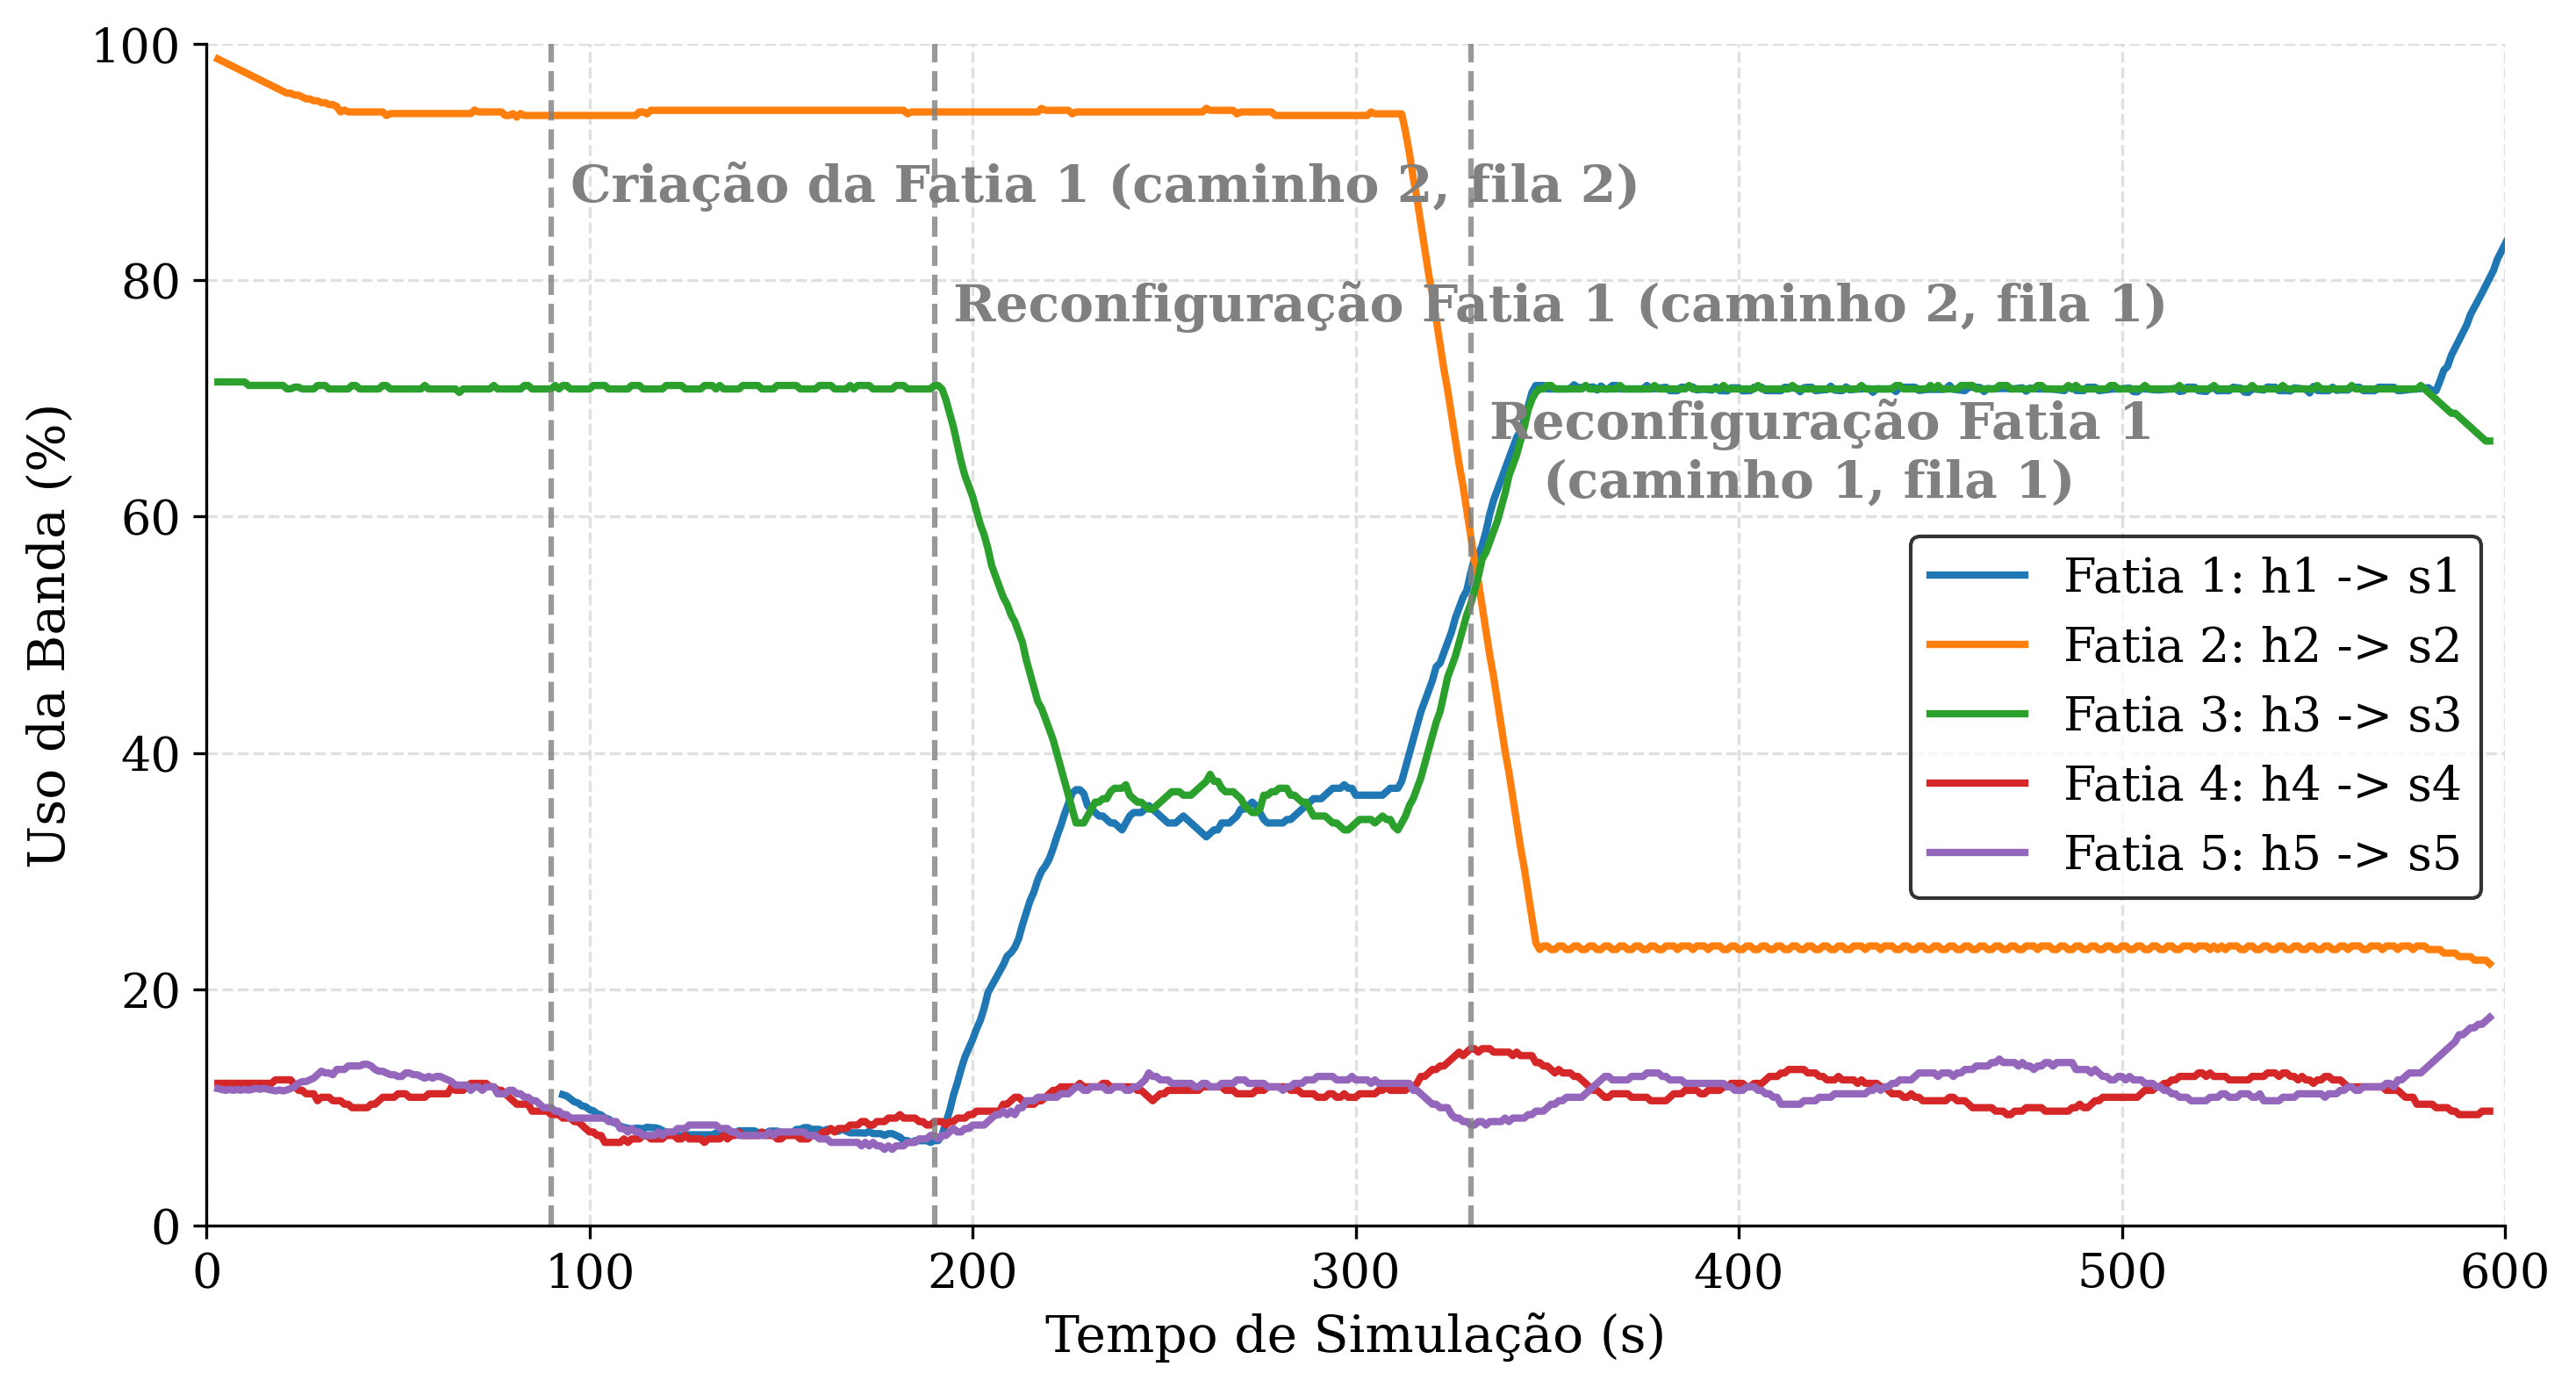
\includegraphics[width=0.85\linewidth]{figuras/grafico_mudanca_caminho_fila_polka.png}
    \caption{Ocupação de banda na segunda rodada do Protótipo 2: reconfiguração concomitante de fila e caminho para a Fatia 1.}
    \label{fig:mininet_mudanca_caminho_fila}
\end{figure}

A dinâmica observada na Figura~\ref{fig:mininet_mudanca_caminho_fila} divide-se em três fases operacionais:
\begin{itemize}
    \item \textbf{Estado inicial e inserção de carga concorrente:} inicialmente, instancia-se a fatia $H_2 \rightarrow S_2$ (Fatia~2) pelo Caminho~1 na Fila~2 --- ocupando praticamente toda a banda disponível (acima de 90\%) devido à ausência de tráfego concorrente naquela rota --- e três fatias pelo Caminho~2: $H_3 \rightarrow S_3$ (Fatia~3) na Fila~1 (70\% de reserva) e os fluxos $H_4 \rightarrow S_4$ e $H_5 \rightarrow S_5$ na Fila~2 (dividindo os 30\% restantes). Em seguida, introduz-se o fluxo $H_1 \rightarrow S_1$ (Fatia~1) pelo Caminho~2 na Fila~2, passando a competir pela reserva de 30\% com $H_4$ e $H_5$.
    \item \textbf{Elevação de prioridade na mesma rota:} na segunda etapa, o nó de borda reconfigura o rótulo da Fatia~1 ($H_1 \rightarrow S_1$) para promovê-la à Fila~1 mantendo o mesmo trajeto (Caminho~2). Como consequência, a Fatia~1 passa a compartilhar equitativamente a reserva de 70\% da Fila~1 com a Fatia~3 ($H_3 \rightarrow S_3$), registrando cerca de 35\% da banda para cada fluxo prioritário.
    \item \textbf{Migração de rota com manutenção de fila prioritária:} por fim, o nó de ingresso altera o \routeID\ da Fatia~1 para desviá-la ao Caminho~1 (\texttt{\{C1, C2, C4, C6\}}), preservando sua atribuição à Fila~1. Essa migração elimina a disputa por recursos críticos sem qualquer intervenção nos nós de núcleo: no Caminho~1, a Fatia~1 passa a usufruir isoladamente dos 70\% de banda da Fila~1, enquanto a Fatia~2 acomoda-se na reserva de 30\% da Fila~2; simultaneamente, no Caminho~2, a Fatia~3 recupera integralmente sua cota de 70\% na Fila~1.
\end{itemize}

% ==============================================================================
\section{Protótipo 3 -- SPolKA em eBPF/XDP sobre Contêineres}
\label{sec:res_prototipo3}

O terceiro protótipo avalia o desempenho do \nome\ diretamente no subsistema de rede do \textit{kernel} Linux (ambiente Containerlab, Figura~\ref{fig:topologia_ebpf}) em enlaces de 1~Gbit/s. Os ensaios submetem o caminho de menor latência ($C_1 \rightarrow C_2 \rightarrow C_4 \rightarrow C_6$, com RTT base de 5~ms) ao envio simultâneo de cinco fluxos concorrentes durante 300 segundos, contemplando duas classes UDP com taxa controlada (Classe~0: \textit{low\_latency} a 2,0~Mbit/s; Classe~1: \textit{critical\_signaling} a 0,3~Mbit/s) e três classes TCP elásticas (\textit{high\_throughput}, \textit{long\_living} e \textit{best\_effort}) parametrizadas conforme as Tabelas~\ref{tab:classes_servico} e~\ref{tab:filas_classe_servico}.

\subsection{Experimento 1 -- Tráfego sem Classificação de Prioridade (FIFO)}
\label{subsec:exp1_fifo}

Nesta primeira rodada de testes, avalia-se o comportamento base da rede operando sob uma disciplina de enfileiramento única do tipo \textit{First-In, First-Out} (FIFO), sem diferenciação ou isolamento entre as classes de serviço.

Os fluxos do protocolo UDP (classes 0 e 1) preservaram integralmente as vazões injetadas, registrando 2,0~Mbit/s e 0,3~Mbit/s com perdas irrelevantes de 0,006\% e 0,002\%, respectivamente. Tal comportamento deve-se à natureza dessas fontes em malha aberta --- desprovidas de controle de congestionamento para desaceleração --- e ao fato de sua carga combinada (2,3~Mbit/s) corresponder a apenas 0,23\% da capacidade do enlace. Contudo, a manutenção da vazão não impediu a degradação da latência: o RTT dessas classes saltou do tempo de propagação base de 5~ms para uma média de 10,49~ms, atingindo picos de 27,9~ms devido ao atraso gerado pelo compartilhamento da fila com o tráfego TCP. Assim, no regime FIFO, a garantia da vazão da classe de baixa latência ocorre à custa de um aumento substancial no atraso.

Por outro lado, as três correntes TCP, reguladas pelo mecanismo de controle de congestionamento CUBIC, responderam às perdas de pacotes (que somaram 19.300 retransmissões) ajustando suas janelas de congestionamento e dividindo de forma equilibrada a capacidade excedente do enlace: 302,2~Mbit/s, 292,5~Mbit/s e 297,9~Mbit/s (Figura~\ref{fig:exp1_fifo}, painel (a)). Isso representa uma variação inferior a 3\% na média do ensaio, embora seus perfis de vazão instantânea tenham apresentado flutuações e alternâncias no decorrer dos 300 segundos de execução. Cabe destacar que, apesar de pertencerem a categorias nominalmente distintas (\texttt{high\_throughput}, \texttt{long\_living} e \texttt{best\_effort}) e estarem associadas a filas separadas nas configurações, a ausência de uma política de escalonamento por classe invalida esses mapeamentos, impondo um tratamento uniforme a todas elas.

\begin{figure}[htbp]
    \centering
    \captionsetup{justification=centering}
    \includegraphics[width=\textwidth]{figuras/exp1_fifo.png}
    \caption{Séries temporais de vazão, \textit{jitter}, RTT e retransmissões no Experimento 1 (regime FIFO com CUBIC).}
    \label{fig:exp1_fifo}
\end{figure}

O painel (b) da Figura~\ref{fig:exp1_fifo} apresenta o \textit{jitter} das duas classes UDP, registrando 0,935~ms para a classe 0 e 2,533~ms para a classe 1. Essa diferença não decorre de tratamento distinto no núcleo da rede --- visto que, sob FIFO, ambas compartilham a mesma fila ---, mas do próprio método de medição. O \textit{jitter}, conforme definido pela RFC~3550, é uma estatística diferencial calculada sobre pacotes consecutivos do fluxo medido, de modo que sua magnitude depende do intervalo entre esses pacotes. Enquanto a classe 0 emite 2.500 pacotes por segundo (espaçamento de 0,4~ms), a classe 1 emite 150 pacotes por segundo (espaçamento de 6,67~ms): pacotes muito próximos encontram a fila em estados correlacionados e produzem estimativas menores de \textit{jitter}, ainda que o atraso sofrido seja idêntico.

\begin{figure}[htbp]
    \centering
    \captionsetup{justification=centering}
    \includegraphics[width=0.9\textwidth]{figuras/exp1_fifo_box.png}
    \caption{Distribuição estatística (\textit{boxplot}) do RTT e \textit{jitter} por classe no Experimento 1 (FIFO).}
    \label{fig:exp1_fifo_box}
\end{figure}

As sondas ICMP, que amostram ambos os caminhos na mesma cadência, confirmam essa equivalência: a variação média do RTT entre amostras consecutivas é de 2,445~ms para a classe 0 e 2,121~ms para a classe 1, com desvios-padrão de 2,97~ms e 2,76~ms, respectivamente. Medidos em igualdade de condições, os dois caminhos apresentam o mesmo comportamento de atraso, conforme também ilustrado na distribuição da Figura~\ref{fig:exp1_fifo_box} (medianas de RTT em 9,90~ms e 9,91~ms para as classes 0 e 1). Conclui-se que, nesta rodada, os valores de \textit{jitter} devem ser interpretados como uma medida absoluta do custo do enfileiramento FIFO para cada fluxo, e não como base de comparação direta entre as classes.

\subsection{Experimento 2 -- Tráfego com Filas de Garantia de Banda (WDRR)}
\label{subsec:exp2_wdrr}

Com o objetivo de priorizar o tráfego e assegurar a reserva de banda direcionada a cada classe de serviço, este ensaio substitui a fila única FIFO pelo algoritmo \textit{Weighted Deficit Round Robin} (WDRR) em todos os nós de transporte da rede. O cenário repete os parâmetros do experimento anterior, alocando uma fila dedicada por classe com reservas de banda (\textit{quanta}) de 60\%, 20\% e 2\% para as classes \texttt{high\_throughput}, \texttt{long\_living} e \texttt{best\_effort}, respectivamente.

\begin{figure}[htbp]
    \centering
    \captionsetup{justification=centering}
    \includegraphics[width=\textwidth]{figuras/exp1_wdrr_cubic.png}
    \caption{Séries temporais de vazão, atraso, retransmissões e ocupação das filas DRR no Experimento 2 (WDRR com CUBIC).}
    \label{fig:exp2_wdrr}
\end{figure}

A diferenciação entre os fluxos manifesta-se de imediato (Figura~\ref{fig:exp2_wdrr}, painel (a)). As três classes elásticas, antes indistinguíveis (302,2~Mbit/s, 292,5~Mbit/s e 297,9~Mbit/s), passam a registrar 505,8~Mbit/s, 284,1~Mbit/s e 85,6~Mbit/s, ordenadas proporcionalmente aos seus respectivos \textit{quanta}. Paralelamente, as classes prioritárias obtêm ganhos expressivos de latência: o RTT médio reduz-se de 10,486~ms para 7,497~ms na classe 0 e de 10,286~ms para 7,366~ms na classe 1. Isso equivale a comprimir o atraso de enfileiramento de 5,49~ms para 2,50~ms --- uma redução superior a 54\% ---, acompanhada pela queda do \textit{jitter} de 0,935~ms para 0,785~ms (classe 0) e de 2,533~ms para 1,939~ms (classe 1). O ônus dessa redistribuição recai sobre a classe \texttt{best\_effort}, que sofre uma retração de 71\% na vazão e tem seu RTT médio elevado de 11,913~ms para 15,462~ms.

\begin{figure}[htbp]
    \centering
    \captionsetup{justification=centering}
    \includegraphics[width=0.9\textwidth]{figuras/exp1_wdrr_cubic_box.png}
    \caption{Distribuição estatística (\textit{boxplot}) do RTT e \textit{jitter} por classe no Experimento 2 (WDRR).}
    \label{fig:exp2_wdrr_box}
\end{figure}

A Tabela~\ref{tab:comparacao_fifo_wdrr} sintetiza os resultados comparativos entre os escalonadores FIFO e WDRR, enquanto a Figura~\ref{fig:exp2_wdrr_box} evidencia a redução das medianas de RTT das classes prioritárias para 6,27~ms e 6,29~ms.

\begin{table}[htbp]
\centering
\caption{Comparação de desempenho entre os escalonadores FIFO e WDRR com o algoritmo CUBIC.}
\label{tab:comparacao_fifo_wdrr}
\begin{tabularx}{\textwidth}{Xccc}
\toprule
\textbf{Métrica / Classe} & \textbf{\shortstack{FIFO\\(\texttt{exp1\_fifo\_cubic})}} & \textbf{\shortstack{WDRR\\(\texttt{exp1\_wdrr\_cubic})}} & \textbf{Variação} \\
\midrule
Classe 0 --- RTT médio        & 10,486~ms    & 7,497~ms     & $-28\%$ \\
Classe 1 --- RTT médio        & 10,286~ms    & 7,366~ms     & $-28\%$ \\
Classe 0 --- \textit{jitter}  & 0,935~ms     & 0,785~ms     & $-16\%$ \\
Classe 1 --- \textit{jitter}  & 2,533~ms     & 1,939~ms     & $-23\%$ \\
Classe 2 ($q=60\%$)           & 302,2~Mbit/s & 505,8~Mbit/s & $+67\%$ \\
Classe 3 ($q=20\%$)           & 292,5~Mbit/s & 284,1~Mbit/s & $-3\%$  \\
Classe 6 ($q=2\%$)            & 297,9~Mbit/s & 85,6~Mbit/s  & $-71\%$ \\
Retransmissões TCP            & 19.300       & 21.969       & $+14\%$ \\
\bottomrule
\end{tabularx}
\fonte{Elaborado pelo autor (2026).}
\end{table}

\subsection{Experimento 3 -- Tráfego com Filas de Garantia de Latência e Banda (SP-WDRR)}
\label{subsec:exp3_sp_wdrr}

Visando atender rigorosamente às classes de serviço sensíveis ao atraso, este ensaio investiga o impacto da adoção de um escalonamento híbrido (SP-WDRR). Mantém-se o WDRR para as classes elásticas com as mesmas definições do Experimento~2, mas promovem-se as classes 0 e 1 a bandas de Prioridade Estrita (\textit{Strict Priority} -- SP), servidas antes de qualquer outra fila, conservando os demais parâmetros inalterados.

\begin{figure}[htbp]
    \centering
    \captionsetup{justification=centering}
    \includegraphics[width=\textwidth]{figuras/exp1_sp-wdrr_cubic.png}
    \caption{Séries temporais de vazão, atraso, retransmissões e ocupação de filas no Experimento 3 (SP-WDRR com CUBIC).}
    \label{fig:exp3_sp_wdrr}
\end{figure}

Os benefícios concentram-se integralmente nas classes prioritárias (Figura~\ref{fig:exp3_sp_wdrr}, painel (b)). O RTT médio decresce de 7,497~ms para 6,054~ms na classe 0 e de 7,366~ms para 5,925~ms na classe 1. Subtraindo-se o tempo de propagação base de 5~ms, observa-se que o atraso de enfileiramento encolhe de 2,50~ms para 1,05~ms (classe 0) e de 2,37~ms para 0,93~ms (classe 1), representando retrações de 81\% e 82\% em comparação ao regime FIFO. Contudo, o aspecto mais significativo reside no comportamento da cauda da distribuição (Figura~\ref{fig:exp3_sp_wdrr_box}): sob o esquema WDRR puro, o RTT máximo da classe 0 havia sofrido degradação em relação ao FIFO (subindo de 27,9~ms para 31,9~ms); com a adoção da prioridade estrita, esse indicador recua para 20,7~ms, enquanto o 95º percentil diminui de 14,0~ms para 9,4~ms (com medianas de 5,29~ms e 5,27~ms). Dessa forma, a previsibilidade observada na média passa a ser assegurada também nos cenários de pior caso --- fator determinante para aplicações críticas de baixa latência.

\begin{figure}[htbp]
    \centering
    \captionsetup{justification=centering}
    \includegraphics[width=0.9\textwidth]{figuras/exp1_sp-wdrr_cubic_box.png}
    \caption{Distribuição estatística (\textit{boxplot}) do RTT e \textit{jitter} por classe no Experimento 3 (SP-WDRR com CUBIC).}
    \label{fig:exp3_sp_wdrr_box}
\end{figure}

Em contrapartida, o impacto sobre as classes elásticas mostra-se marginal. Como as classes promovidas possuem banda estritamente limitada por contrato (2,0~Mbit/s e 0,3~Mbit/s, totalizando apenas 0,23\% da capacidade do enlace), seu atendimento prioritário consome uma fração mínima dos recursos. Essa delimitação viabiliza o uso seguro da prioridade estrita, mitigando o risco de inanição (\textit{starvation}) tipicamente associado a fluxos privilegiados sem restrição de taxa. Consequentemente, a classe \texttt{high\_throughput} preserva seus 505,8~Mbit/s, enquanto \texttt{long\_living} e \texttt{best\_effort} sofrem reduções pontuais de 1,3\% (para 280,5~Mbit/s) e 6,5\% (para 80,1~Mbit/s), respectivamente. No agregado, a vazão conjunta das três classes recua apenas 1,0\%, passando de 875,5~Mbit/s para 866,4~Mbit/s.

\subsection{Experimento 4 -- Impacto do Controle de Congestionamento BBR sob SP-WDRR}
\label{subsec:exp4_bbr}

Este experimento avalia o desempenho do algoritmo de controle de congestionamento BBR (\textit{Bottleneck Bandwidth and Round-trip propagation time}) em comparação ao CUBIC, replicando integralmente a topologia e a disciplina de filas SP-WDRR do Experimento~3.

\paragraph{Fundamentação dos algoritmos avaliados}
O algoritmo CUBIC, baseado em perda, incrementa a janela de congestionamento por meio de uma função cúbica até detectar o descarte de pacotes, momento em que aplica uma redução multiplicativa. Por depender do esgotamento do \textit{buffer} para identificar o congestionamento, o CUBIC tende a saturar as filas antes de reduzir a taxa de transmissão, gerando oscilações periódicas (padrão dente de serra) e acúmulo de atraso. Em contrapartida, o BBR, baseado em modelo, estima continuamente a largura de banda máxima do gargalo (\textit{BtlBw}) e o menor RTT de propagação (\textit{RTprop}). Em vez de reagir a perdas, o BBR ajusta a cadência de envio para manter o volume de dados em trânsito próximo ao produto banda-atraso (BDP), realizando sondagens periódicas de banda (ciclo de ganho) e reduções temporárias de taxa para recalibrar o RTT mínimo (\textit{ProbeRTT}). Enquanto o CUBIC utiliza a ocupação do \textit{buffer} como sinal de controle, o BBR busca operar no ponto ótimo da curva vazão-atraso, minimizando o enfileiramento.

\begin{figure}[htbp]
    \centering
    \captionsetup{justification=centering}
    \includegraphics[width=\textwidth]{figuras/exp1_sp-wdrr_bbr.png}
    \caption{Séries temporais de vazão, atraso, retransmissões e ocupação de filas no Experimento 4 (SP-WDRR com BBRv1).}
    \label{fig:exp4_bbr}
\end{figure}

\paragraph{Análise dos resultados}
Substituindo o CUBIC pelo BBR\footnote{Embora o protocolo BBR já se encontre em sua terceira revisão (rascunho IETF em \url{https://datatracker.ietf.org/doc/draft-ietf-ccwg-bbr/}), esta avaliação emprega a versão 1 (BBRv1), por ser a implementação nativamente disponível e consolidada no kernel Linux~6.8 utilizado no ambiente experimental.} nos três fluxos TCP nesta rodada, a assinatura característica do algoritmo manifesta-se prontamente no painel (a) da Figura~\ref{fig:exp4_bbr}: em vez de oscilarem e alternarem posições --- comportamento típico do CUBIC ---, as vazões estabilizam-se em torno de patamares bem definidos. Essa estabilidade decorre da cadência controlada de transmissão (\textit{pacing}), que evita o ciclo contínuo de preenchimento e esvaziamento dos \textit{buffers}.

\begin{figure}[htbp]
    \centering
    \captionsetup{justification=centering}
    \includegraphics[width=0.9\textwidth]{figuras/exp1_sp-wdrr_bbr_box.png}
    \caption{Distribuição estatística (\textit{boxplot}) do RTT e \textit{jitter} por classe no Experimento 4 (SP-WDRR com BBRv1).}
    \label{fig:exp4_bbr_box}
\end{figure}

Com essa alteração, a vazão agregada atingiu 890,6~Mbit/s, ante os 866,4~Mbit/s registrados com CUBIC ($+2,8\%$). Paralelamente, observou-se redução do RTT médio em todos os fluxos TCP: a classe \texttt{high\_throughput} caiu de 11,20~ms para 10,32~ms; a \texttt{long\_living}, de 12,12~ms para 10,88~ms; e a \texttt{best\_effort}, de 14,21~ms para 13,62~ms. Esse ganho de vazão concentrou-se na classe com maior \textit{quantum}, cuja taxa subiu de 505,8~Mbit/s para 564,6~Mbit/s ($+11,6\%$), enquanto as duas outras classes apresentaram retrações de aproximadamente 9\% cada.

Por outro lado, houve um acréscimo expressivo de 159\% nas retransmissões TCP, que subiram de 24.482 para 63.403 pacotes, com a classe \texttt{high\_throughput} respondendo por 49.350 desse total (0,34\% dos segmentos transmitidos). Esse fenômeno é condizente com as premissas do BBRv1, que não toma descartes como indicativo direto de congestionamento, preservando a vazão estimada. Por fim, as classes prioritárias sustentaram o patamar mínimo de latência da rota --- com RTT médio de 5,96~ms em ambas, 95º percentil de 8,70~ms e 8,80~ms (Figura~\ref{fig:exp4_bbr_box}) e \textit{jitter} inferior ao obtido com CUBIC (0,789~ms e 1,439~ms) ---, embora a taxa de perda na classe 0 tenha se elevado de 0,011\% para 0,100\%. A Tabela~\ref{tab:comparacao_cubic_bbr} consolida a comparação direta entre os dois algoritmos de controle de congestionamento sob o regime SP-WDRR.

\begin{table}[htbp]
\centering
\caption{Comparação de desempenho entre os algoritmos CUBIC e BBRv1 sob escalonamento SP-WDRR.}
\label{tab:comparacao_cubic_bbr}
\begin{tabularx}{\textwidth}{Xccc}
\toprule
\textbf{Métrica / Fluxo} & \textbf{CUBIC} & \textbf{BBRv1} & \textbf{Variação} \\
\midrule
Vazão Classe 2 ($q=45.000$~B)     & 505,8~Mbit/s & 564,6~Mbit/s & $+11,6\%$ \\
Vazão Classe 3 ($q=15.000$~B)     & 280,5~Mbit/s & 253,2~Mbit/s & $-9,7\%$  \\
Vazão Classe 6 ($q=1.500$~B)      & 80,1~Mbit/s  & 72,8~Mbit/s  & $-9,1\%$  \\
Vazão agregada (fluxos elásticos) & 866,4~Mbit/s & 890,6~Mbit/s & $+2,8\%$  \\
Retransmissões TCP totais         & 24.482       & 63.403       & $+159\%$  \\
RTT médio TCP (c2 / c3 / c6)      & 11,20 / 12,12 / 14,21~ms & 10,32 / 10,88 / 13,62~ms & Redução geral \\
RTT médio UDP (c0 / c1)           & 6,054 / 5,925~ms & 5,964 / 5,963~ms & Equivalente \\
\textit{Jitter} médio UDP (c0 / c1) & 0,872 / 1,806~ms & 0,789 / 1,439~ms & Melhoria \\
Taxa de perda Classe 0            & 0,011\%      & 0,100\%      & Aumento de $9\times$ \\
\bottomrule
\end{tabularx}
\fonte{Elaborado pelo autor (2026).}
\end{table}

% ==============================================================================
\section{Síntese e Discussão dos Resultados}
\label{sec:sintese_resultados}

A análise conjunta dos três protótipos evidencia a evolução progressiva do controle de Qualidade de Serviço proporcionada pela arquitetura \nome\ sem comprometer a escalabilidade do núcleo sem estado (\textit{stateless}):

\begin{enumerate}
    \item \textbf{Granularidade de controle:} enquanto o Protótipo~1 (\polka\ original) demonstra que o roteamento na origem em hardware Tofino isola fluxos mediante a migração entre túneis disjuntos, o \nome\ (Protótipos~2 e~3) expande essa capacidade ao permitir a diferenciação de múltiplas classes de serviço dentro de um mesmo caminho físico por meio da codificação conjunta do \portID\ e do \qID\ no rótulo \routeID.
    \item \textbf{Agilidade e ausência de estado no núcleo:} nos três ambientes avaliados (Tofino/freeRtr, P4/BMv2 e eBPF/XDP), todas as reconfigurações de rota e promoções de fila foram executadas exclusivamente pela atualização de regras nos nós de borda, sem necessidade de sinalização ou alteração de tabelas nos comutadores intermediários.
    \item \textbf{Compromisso entre latência, vazão e controle de congestionamento:} os ensaios no Protótipo~3 comprovam que o escalonamento híbrido SP-WDRR reduz o atraso de enfileiramento das classes críticas em mais de 80\% em relação ao FIFO (mantendo o 95º percentil abaixo de 9,5~ms), ao mesmo tempo em que preserva a proporção de banda contratada entre as fatias elásticas. Ademais, a combinação de SP-WDRR com o algoritmo BBRv1 estabiliza a vazão instantânea dos fluxos TCP e eleva a utilização agregada do enlace, embora exija atenção ao aumento de retransmissões inerente à menor sensibilidade a perdas dessa versão do protocolo.
\end{enumerate}